\subsection{条件分布的改善与完整轨迹的改善}

在固定长度 $H$ 的 autoregressive 模型中，记完整序列分布为 $Q(y)=\prod_iq(y_i\mid y_{<i})$、$T(y)=\prod_it(y_i\mid y_{<i})$。KL 链式法则给出
\begin{equation}
 \KL(Q\Vert T)=\sum_{i=1}^H\E_{s_i\sim Q}\KL(q(\cdot\mid s_i)\Vert T(\cdot\mid s_i)).
 \label{eq:proximal-sequence-chain}
\end{equation}
更新每个条件分布后，访问测度也从 $Q$ 变成 $P$。因此逐个 prefix 的条件 KL 下降，不足以让这条随策略改变权重的总和下降。本书固定测度问题明确冻结权重；序列混合与逐 token 混合是不同算子。

\paragraph{一个两步、完整支持的反例。}
第一步取 $q_0=(0.99,0.01)$、$T_0=(0.01,0.99)$。第一分支的第二步取 $q_A=T_A=(1/2,1/2)$；第二分支取 $q_B=(1-10^{-6},10^{-6})$、$T_B=(10^{-30},1-10^{-30})$。在全部三个条件分布上同时执行精确幂均值步，$\eta=0.1$。每个条件 KL 都下降或保持零，但完整序列的 reverse KL 为
\begin{center}
\begin{tabular}{lrr}
\toprule
形状 & 更新前完整序列 KL & 更新后完整序列 KL\\
\midrule
$\kappa=0$ & 5.19399 & 6.07445\\
$\kappa=1/2$ & 5.19399 & 7.09792\\
$\kappa=1$ & 5.19399 & 10.44581\\
\bottomrule
\end{tabular}
\end{center}
数值由 \path{results/power-mean-20261013/generalization-checks.json} 的完整精度记录为准。变化的原因是学生更频繁进入尚未拟合好的第二分支。算术形状将该分支概率从 $0.01$ 提升到 $0.108$，其条件误差仍然很大。保持原访问权重的条件 KL 总和却从 $5.19399$ 降到 $4.38503$；两种测度给出不同结论。这个反例在固定两步时域已成立，不依赖 EOS 或长度归一化。

\begin{figure}[htbp]
 \centering
 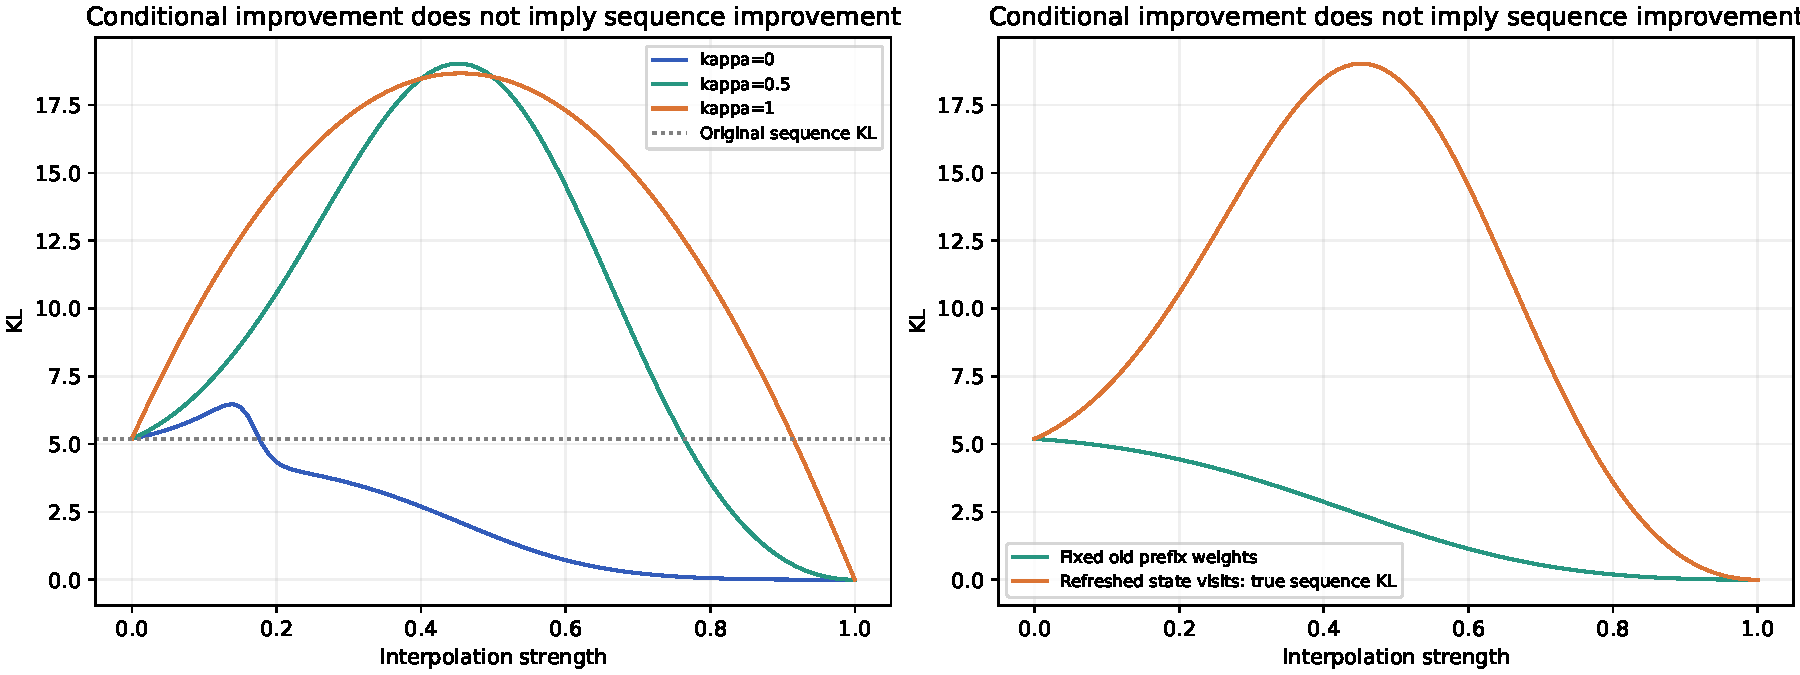
\includegraphics[width=\textwidth]{../../results/power-mean-20261013/sequence-scope-counterexample.pdf}
 \caption{精确条件更新仍可能使完整序列 KL 上升。左图比较三种形状；右图固定平方根形状，对照冻结旧 prefix 权重的条件目标与更新后访问测度下的真实序列 KL。}
\end{figure}

\subsection{序列混合的条件概率包含额外因子}

对序列层面的算术混合 $M=(1-\eta)Q+\eta T$，条件分布为
\begin{equation}
 M(a\mid s)=(1-\eta_s)q(a\mid s)+\eta_st(a\mid s),\qquad
 \eta_s=\frac{\eta T(s)}{(1-\eta)Q(s)+\eta T(s)}.
\end{equation}
它的 teacher 权重依赖已经生成的 prefix。固定 $\eta$ 的逐 token 算术混合因此一般不同于序列层面的算术混合。

对序列几何 target $M(y)\propto Q(y)^{1-\eta}T(y)^\eta$，定义后缀配分函数
\begin{equation}
 Z_\eta(s)=\sum_zQ(z\mid s)^{1-\eta}T(z\mid s)^\eta.
\end{equation}
将带前缀 $s$ 的序列质量先求和再作条件化，得到
\begin{equation}
 M(a\mid s)=q(a\mid s)^{1-\eta}T(a\mid s)^\eta
 \frac{Z_\eta(sa)}{Z_\eta(s)}.
\end{equation}
逐 token 几何 target 忽略了 action 相关的后缀配分函数；它只有在这些后缀因子与 action 无关时才恢复完整序列 target。两个端点都展示了条件化与混合一般不能交换。

\subsection{真实序列 reverse KL 的一阶方向}

记 suffix 值 $V^q(s)=\KL(Q(\cdot\mid s)\Vert T(\cdot\mid s))$。链式法则给出递推
\begin{equation}
 V^q(s)=\E_{a\sim q(\cdot\mid s)}[\log(q(a\mid s)/T(a\mid s))+V^q(sa)],
\end{equation}
终点的值为零。完整序列 KL 的 policy gradient 是
\begin{equation}
 \nabla\KL(Q\Vert T)
 =\E_Q\sum_i\psi_i\sum_{j\ge i}\log\frac{q(y_j\mid s_j)}{T(y_j\mid s_j)}.
\end{equation}
推导时，$\nabla\log Q=\sum_i\psi_i$，直接微分 KL 多出的 $\E_Q\nabla\log Q$ 为零；过去 reward 与当前 score 的乘积则因条件零均值而消失。对某个 prefix 的局部方向，未来成本不能省略；其负信号是
\begin{equation}
 f_{\mathrm{seq}}^q(s,a)=\log\frac{T(a\mid s)}{q(a\mid s)}-V^q(sa).
\end{equation}
条件中心化后，它给出真实序列 reverse KL 的自然梯度方向。即时 log-ratio 的固定测度优化只保留第一项。长度平均的未来 return、随机组标准化或其他信号变换需要另行解释其目标，不能直接继承这条精确 policy gradient。

若直接在有限序列空间构造幂均值 target，前面的凸生成散度与矩定理仍然成立。该空间虽有指数级的序列数，归一化的二阶矩界不含空间大小。若每个 token score 范数不超过 $S$，$H$ 有限，则序列 score 范数不超过 $HS$，对应的梯度二阶矩界只增加 $H^2S^2$ 因子。序列 target 的表达、采样和投影是不同问题；固定 prefix 理论与任务正确率是不同证据，须分别报告。
